\documentclass[thesis]{deutez}
%%My_library 
\usepackage{placeins}%resim kaymaları için kullanıldı
\usepackage{amsmath,amsthm,mathtools}
%%Images
\graphicspath{ {/home/rabikkk/Pictures/images/} }

%-------------------------------------%%

\watermarklogo{Deu.jpg}  % Dokuz Eylül Üniversitesi Logosu; Sayfaya arkasına varsayılan logo olarak basılır.
\projectname{Smart Mirror Controller}%
\ogrencininadi{Rabia DOĞAN}%
\advisor{Ph.D. Özgür TAMER}%
\jurya{Prof. Dr. Gülay TOHUMOĞLU}
\juryb{Ph.D. Abdül BALIKCI}
\chair{Prof. Dr. Mehmet KUNTALP}
\time{January,2021}%

\begin{document}

\begin{abstract}
		
\end{abstract}

\begin{ozet}
	
\end{ozet}
 
\tableofcontents
\listoftables
\listoffigures

\start

\chapter{INTRODUCTION}

\chapter{TECHNICAL BACKGROUND}

\section{Introduction to Artificial Neural Networks}
\section{Learning Process of Artificial Neural Networks}

\chapter{MATERIALS AND METHODS}
\section{Dataset}
\section{Data Augmentation}
\section{Model Architecture for LE-NET5}
\chapter{PROGRESS AND RESULT}
\section{Capture Thermopiles Image}
\subsection{Heimann Thermopile Array Sensor communication}
First, I provided the connections between the sensor and the Raspberry Pi in order to receive the image. I provided the communication with the mini card I made in 4.2 using the I2C protocol.

With the device connected to a Raspberry Pi, and with the Pi configured.\cite{adaf} correctly for I2C, I was able to see the devices connected with the i2cdetect command.
\begin{figure}[h!]
	\centering
	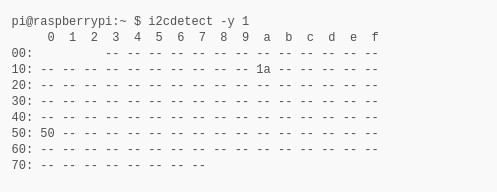
\includegraphics[width=0.8\textwidth]{raspi1.png}
	\caption{Thermopile Infrared Array Device and EEPROM Addresses}
\end{figure}
\FloatBarrier

In order to be able to read the data properly, the python-periphery\cite{perip} library was used. The sensor is divided into two parts (Top and Bottom Half), which are also divided into 4 blocks. The reading order is shown below for different blocks. When a conversion is initiated, the X Block of the upper and lower half are measured simultaneously. Each block consists of 128 Pixels sampled entirely in parallel. The reading order in the lower half is mirrored compared to the upper half so the center lines are always read last.

	\begin{table}[h!]
	\begin{center}
		\caption{Read Data 1 Command (Top Half of Array)}
		\begin{tabular}{|c|c|c|c|c|c|c|c|c|} 
			\hline
			Addr/CMD & \multicolumn{8}{c|}{0x1A (7 Bit!) / 0x0A}\\\cline{1-9}
			Read Data &7&6&5&4&3&2&1&0\\
			\cline{1-9}
			1. Byte / 2. Byte & \multicolumn{8}{c|}{PTAT 1 MSB / LSB or Vdd 1 MSB / LSB}\\\cline{1-9}
			3. Byte / 4. Byte & \multicolumn{8}{c|}{Pixel (0+BLOCK*128) MSB / LSB}\\\cline{1-9}
			5. Byte / 6. Byte & \multicolumn{8}{c|}{Pixel (1+BLOCK*128) MSB / LSB}\\\cline{1-9}
			... & \multicolumn{8}{c|}{}\\\cline{1-9}	
			257. Byte / 258. Byte & \multicolumn{8}{c|}{Pixel (127+BLOCK*128) MSB / LSB}\\\cline{1-9}
			
		\end{tabular}
	\end{center}
\end{table}
\FloatBarrier
\begin{table}[h!]
	\begin{center}
		\caption{Read Data 2 Command (Bottom Half of Array)}
		\begin{tabular}{|c|c|c|c|c|c|c|c|c|} 
			\hline
			Addr/CMD & \multicolumn{8}{c|}{0x1A (7 Bit!) / 0x0B}\\\cline{1-9}
			Read Data &7&6&5&4&3&2&1&0\\
			\cline{1-9}
			1. Byte / 2. Byte & \multicolumn{8}{c|}{PTAT 2 MSB / LSB or Vdd 2 MSB / LSB}\\\cline{1-9}
			3. Byte / 4. Byte & \multicolumn{8}{c|}{Pixel (992-BLOCK*128) MSB / LSB}\\\cline{1-9}
			5. Byte / 6. Byte & \multicolumn{8}{c|}{Pixel (993-BLOCK*128) MSB / LSB}\\\cline{1-9}
			... & \multicolumn{8}{c|}{}\\\cline{1-9}	
			65. Byte / 66. Byte & \multicolumn{8}{c|}{Pixel (1023-BLOCK*128) MSB / LSB}\\\cline{1-9}
			
			65. Byte / 66. Byte & \multicolumn{8}{c|}{Pixel (1023-BLOCK*128) MSB / LSB}\\\cline{1-9}
			
			67. Byte / 68. Byte & \multicolumn{8}{c|}{Pixel (960-BLOCK*128) MSB / LSB}\\\cline{1-9}
			
			69. Byte / 70. Byte & \multicolumn{8}{c|}{Pixel (961-BLOCK*128) MSB / LSB}\\\cline{1-9}
			
			... & \multicolumn{8}{c|}{}\\\cline{1-9}
			
			129. Byte / 130. Byte & \multicolumn{8}{c|}{Pixel (991-BLOCK*128) MSB / LSB}\\\cline{1-9}
			
			131. Byte / 132. Byte & \multicolumn{8}{c|}{Pixel (928-BLOCK*128) MSB / LSB}\\\cline{1-9}
			
			...& \multicolumn{8}{c|}{}\\\cline{1-9}
			
			257. Byte / 258. Bytes& \multicolumn{8}{c|}{Pixel (927-BLOCK*128) MSB / LSB}\\\cline{1-9}
			
		\end{tabular}
	\end{center}
\end{table}
\FloatBarrier
Each block is checked before it is read. The python-opencv\cite{cv2} library was used to visualize the obtained result.
\begin{figure}[h!]
	\centering
	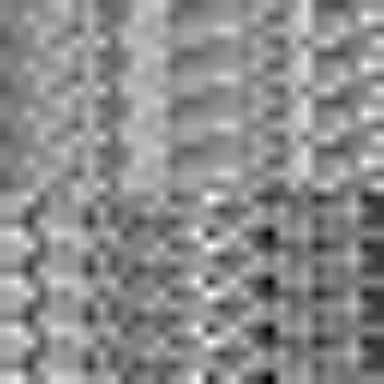
\includegraphics[width=0.23\textwidth]{4.img}
	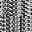
\includegraphics[width=0.23\textwidth]{3.img}
	\caption{Thermal Image}
\end{figure}
\FloatBarrier


Each pixel (or each analog-to-digital converter, given the repeating structure corresponding to each "block" of the sensor) has its own offset and sensitivity to incident light. Without calibrating it, this constant "noise" suppresses the signal from changing IR/temperature conditions. By subtracting the two frames in quick succession, this common noise signal is removed.

However, it is still quite noisy, as this frame subtraction increases random noise (since we now have contributions from two frames) and does not correct pixel-dependent sensitivity.
Only fabrication calibration will be done with EEPROM data in the next step.

\subsection{Calibrating images from Heimann Thermopile Array Sensor}

After reading an image off a Heimann thermopile array, the pixel values can be converted to temperature readings through the use of calibration parameters stored on the device. To extract the calibration parameters, it is easiest to first read off the entire EEPROM on the thermopile array.

\begin{figure}[h!]
	\centering
	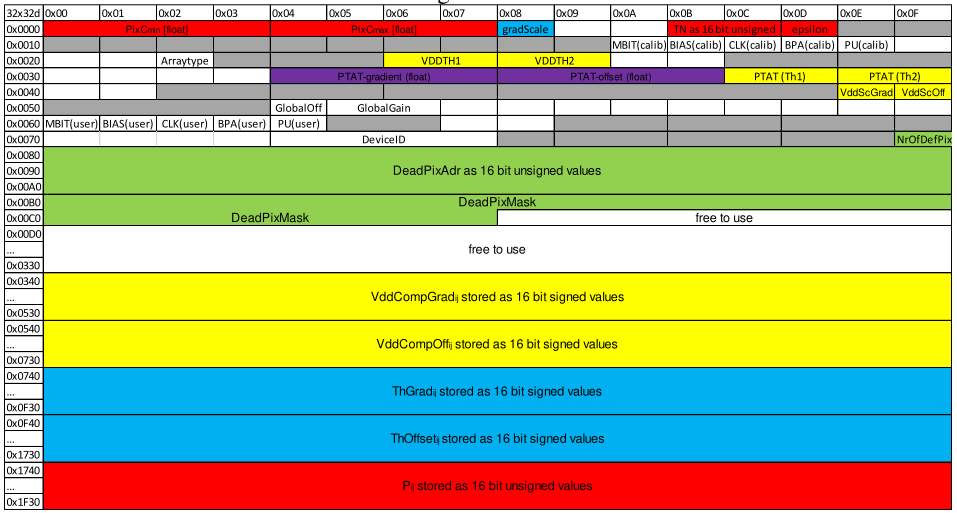
\includegraphics[width=1\textwidth]{eeprom}
	\caption{EEPROM overview 32x32d\cite{datasheet}}
\end{figure}
\FloatBarrier
Then, parameters and calibration values can be extracted from this array, as described in the Heimann datasheet.\cite{datasheet}\\
Calibration for only one pixel is done as follows.\\
$PTAT_{av} = \frac{\sum \limits _{i=0}^{7}{PTAT_i}}{8}=38152 Digits $ \\
$PTAT_{gradient}=0.0211 dK/Digit $ and $PTAT_{offset}=2195.0dK$ \\
$ V_{00}=34435 Digits $\\
$ elOffset[0]=34240 $\\
$gradScale=24  $\\
$ThGrad_{00}=11137$ \\
$ThOffset_{00}=65506 $\\
$VDD_{av}=35000 $\\
$ VDD_{TH1}= 33942 $\\
$ VDD_{TH2} = 36942 $\\
$ PTAT_{TH1} = 30000  $\\
$ PTAT_{TH_2} = 42000  $\\
$ VddCompGrad[ 0 ] = 10356 $\\
$ VddCompOff[ 0 ] =51390  $\\
$ VddScGrad = 16 $\\
$VddScOff = 23  $\\
$ PixC_{00}= 1\cdot087\cdot10^8 $\\
$ PCSCALEVAL = 1\cdot10^8 $\\
Calculation of ambient temperature:\\
$ 	T_a=PTAT_{av} \cdot PTAT_{gradient}+ PTAT_{offset}=38152 \cdot 0.0211 + 2195.0 dK =3000 dK $\\
Compensation of thermal offset:\\
$V_{00\_Comp}=V_{00}-\frac{Th_{Grad00} \cdot T_a}{2^{gradScale}}-Th_{Offset_{00}}=34439 $\\
Compensation of electrical offset:\\
$ 	V_{00\_Comp}^{\ast} =V_{00\_Comp}-elOffset[0]=199 $\\
Compensation of supply voltage:\\
$ V_{00-VDD_{Comp}}=V_{00\_Comp}^{\ast}-\frac{\frac{Vdd_{CompGrad}[0]\cdot PTAT_{av}}{2^{Vdd_{ScGrad}}}+V_{Vdd_{Compoff}}[0]}{2^{Vdd_{ScOff}}}\\
	\cdot(VDD_{av}-VDD_{TH1}-(\frac{VDD_{TH2}-VDD_{TH1}}{PTAT_{TH2}-PTAT_{TH1}})\cdot(PTAT_{av}-PTAT_{TH1}))=199-1=198 $
The sensitivity coefficients ( PixC ij ) are calculated:\\
$PixC_{00}=(\dfrac{P_{00} \cdot (PixC_{Max}-PixC_{Min})}{65535}+PixC_{Min}) \cdot \frac{epsilon}{100} \cdot \frac{GlobalGain}{100000}=1\cdot087\cdot10^8 $\\
Leading to a compensation of the pixel voltage:\\
$V_{00PixC}=\dfrac{	V_{00-VDD_{Comp}}\cdot PCSCALEVAL}{PixC_{0}}=182$\\ 

All operations are applied for 1024 pixels. Application result images are as in figure 4.4.

\begin{figure}[h!]
	\centering
	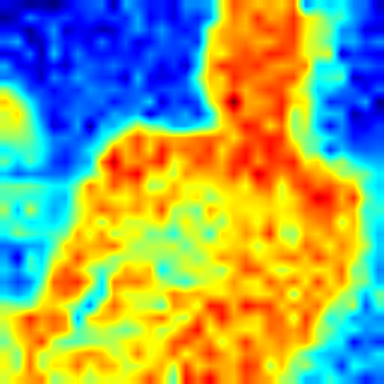
\includegraphics[width=0.23\textwidth]{last_test58}
	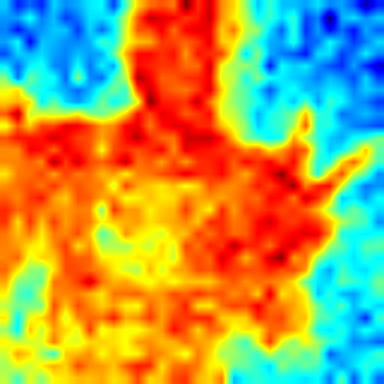
\includegraphics[width=0.23\textwidth]{last_test59}
	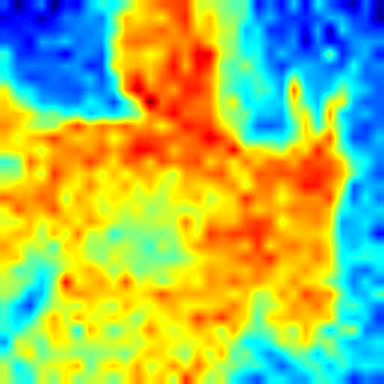
\includegraphics[width=0.23\textwidth]{last_test60}
	\caption{Thermal Images with EEPROM Calibration Data}
\end{figure}
\FloatBarrier
\paragraph~	\textbf{NOTE:All steps to acquired the image are made with reference to the datasheet\cite{datasheet}.}
\section{Hand Thermal Image Isolation}
The hand was isolated from the background without using any image processing method. For this, it has been arranged in a way that can remove the ambient temperature of the device from the image before giving a command. First, the average of 10 images was taken and given to all images. Thus, the background temperature was isolated.
\begin{figure}[h!]
	\centering
	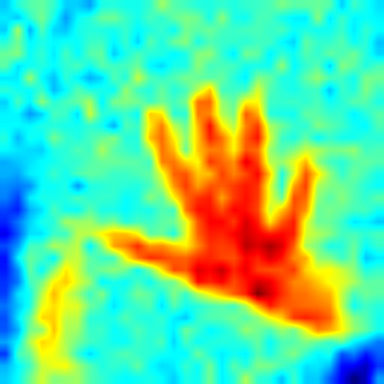
\includegraphics[width=0.23\textwidth]{rgb0}
	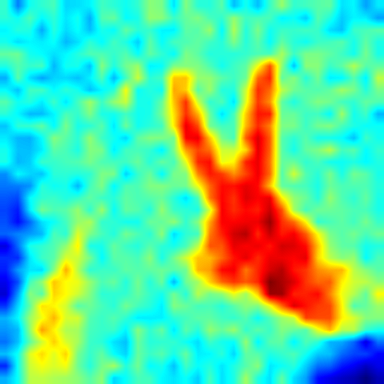
\includegraphics[width=0.23\textwidth]{rgb1}
	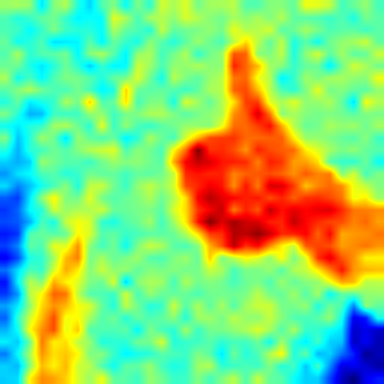
\includegraphics[width=0.23\textwidth]{rgb2}
	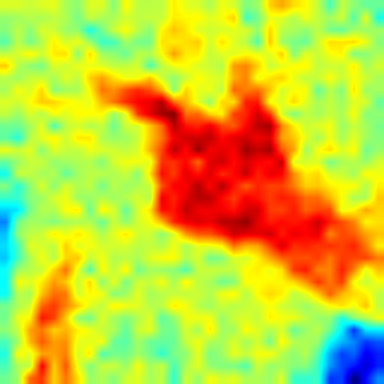
\includegraphics[width=0.23\textwidth]{rgb3}
	\caption{Thermal Images with Background}
\end{figure}
\section{Hand Gesture Recognition}
\subsection{Static Gesture Recognition}
\subsection{Dynamic Gesture Recognition}
\section{Sensor and MCU Communication PCB Design}
A sensor PCB design will be made with the selection and supply of the passive infrared sensor. In the PCB design in question, a schematic design will be made first and the necessary components and connections will be made schematically. After this part, the schematic design will be turned into a printed circuit. In the design of the printed circuit board, along with the schematic design, the physical properties of the place where the sensor will be mounted will be taken into consideration in the current smart mirror design. After this part, the designed sensor PCB will be produced in an external company and its assembly will be carried out in the company.\\
The pcb and schematic drawings of the communication PCB are as shown in the figures below. Schematic and PCB design will be done using KiCad EDA - Schematic Capture \& PCB Design Software. In the next step, support will be received for printed circuit operations. After soldering the printed cards, our sensor communication PCB will be ready and the test phase will begin. \\
\begin{figure}[h!]
	\centering
	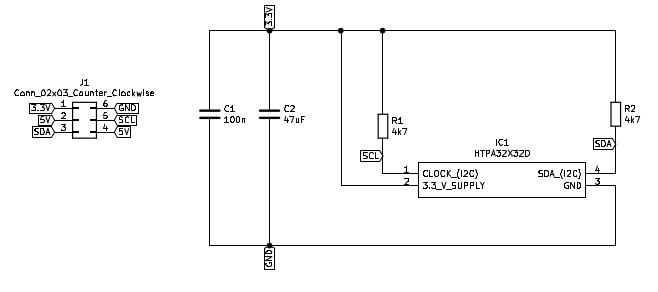
\includegraphics[width=0.7\textwidth]{schematic}
	\caption{Schematic Design of Communication PCB}
\end{figure}
\FloatBarrier
\begin{figure}[h!]
	\centering
	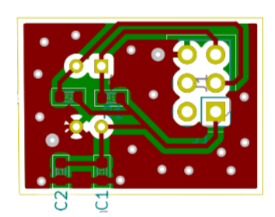
\includegraphics[width=0.4\textwidth]{pcb}
	\caption{PCB Design of Communication PCB}
\end{figure}
\FloatBarrier
\section{Matching Gesture to Commands of Smart Mirror}
\chapter{COST ANALYSIS}
\chapter{CONCLUSION}
\bibliographystyle{deueeebst2.bst}
\bibliography{fp_refs}
\chapter{APPENDIX}

\end{document}